\subsection{Exercise 26.4}

\noindent \hspace{1.2em}\textit{Find the absolute maximum value and the absolute minimum value of the following functions (Question 1 to 3):}
\begin{enumerate}
    \item $f(x)=5-36 x+3 x^2+4 x^3$, $[-1,2]$
    \item $f(x)=4 x^2\left(x^2-2\right)$, $[-1,3]$
    \item $f(x)=x^5-5 x^4+5 x^3$, $[0,4]$
    \item A metal wire with a length of $60$cm is bent into a rectangle. Find the width
          and the length of the rectangle so that the area of the rectangle is the
          largest.
    \item A metal wire with a length of $100$cm is cut into two sections. Each section is
          bent into a square. Find the length of these two sections of the wire so that
          the sum of the areas of the two squares is the smallest.
    \item As shown in the diagram below, a trapezium has three sides of length $10$cm.If
          the area of the trapezium is the largest, find the length of the fourth side.
          Hence, find the maximum area of the trapezium.
          \begin{center}
              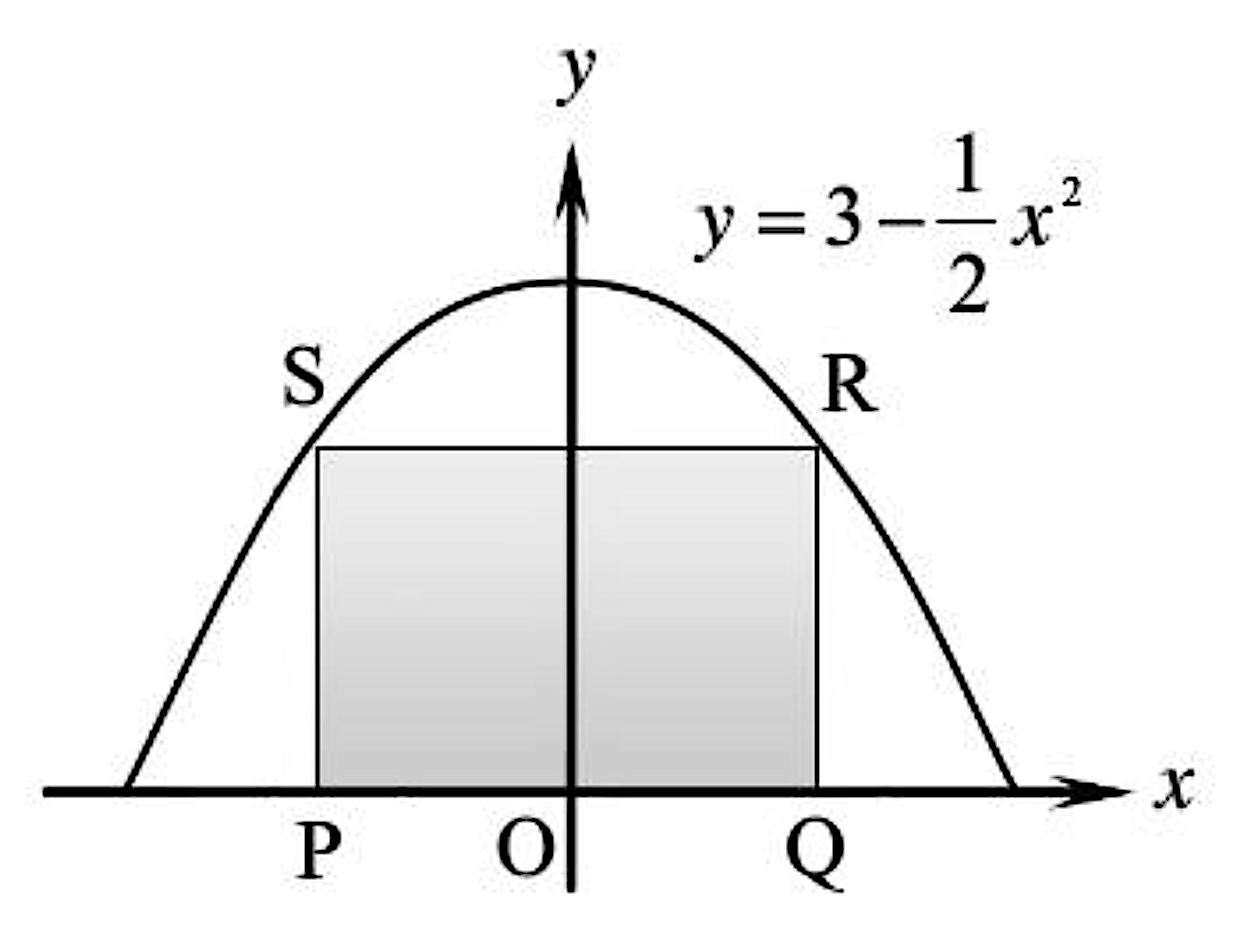
\includegraphics[scale=0.25]{assets/26-9.png}
          \end{center}
    \item A right cone has a slant height of $9$cm. Find the height of the cylinder such
          that the volume of the cylinder is the largest.
    \item A cylinder shaped can with lid has a volume of $250\pi$cm$^3$. Find the bottom
          radius and the height of the can so that the material used is the least.
    \item Split the number 20 into two parts such that one part is 4 times the reciprocal
          of another part, and the the sum of it with with 9 times the reciprocal of
          another part is the smallest.
    \item A metal wire with a length of $150$cm is split into two sections, and they are
          bent into a square and a circle respectively. Find the length of these two
          sections such that the sum of the area of the square and the circle is the
          smallest.
    \item As shown in the diagram below, a window is formed by a rectangle and a
          semicircle. The perimeter of the entire window is 300cm. If the area of the
          window is the largest, find the length of the rectangle. Hence, find the
          maximum area of the window.
          \begin{center}
              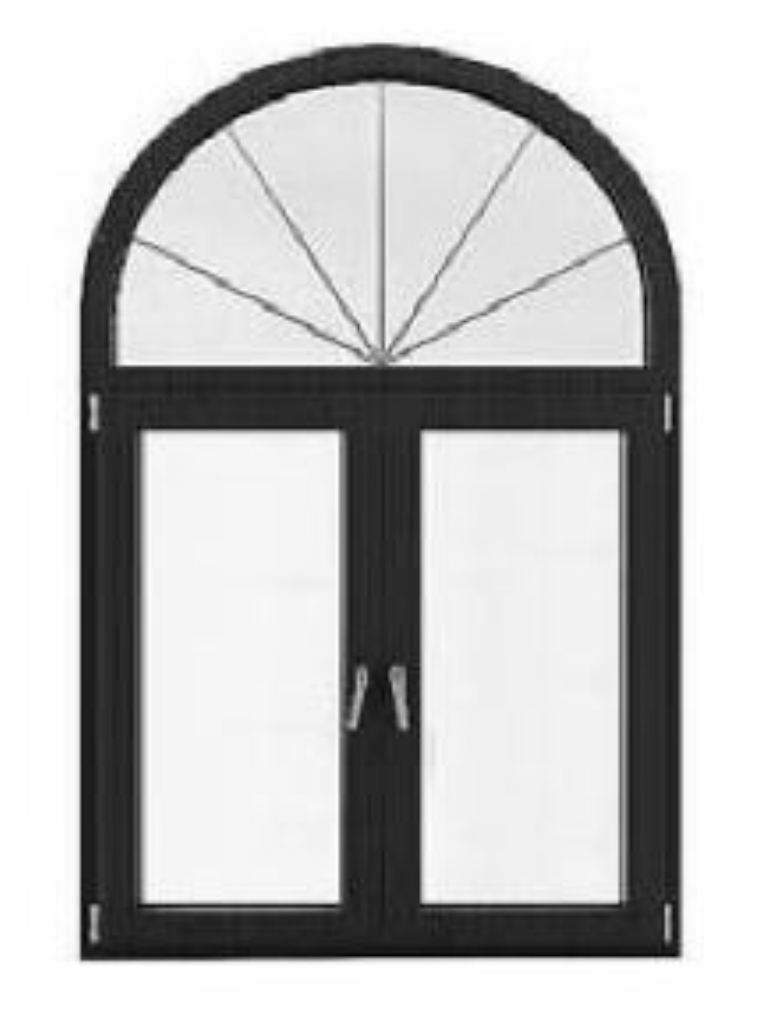
\includegraphics[scale=0.25]{assets/26-10.png}
          \end{center}
    \item In the diagram below, $PQRS$ is a rectangle, the coordinates of $P$ and $Q$ are
          $(-k, 0)$ and $(k, 0)$ respectively, where $k > 0$, and the two points $R$ and
          $S$ are on the curve $y = 3- \dfrac{1}{2}x^2$. Find the value of $k$ such that
          the area of the rectangle is the largest.
          \begin{center}
              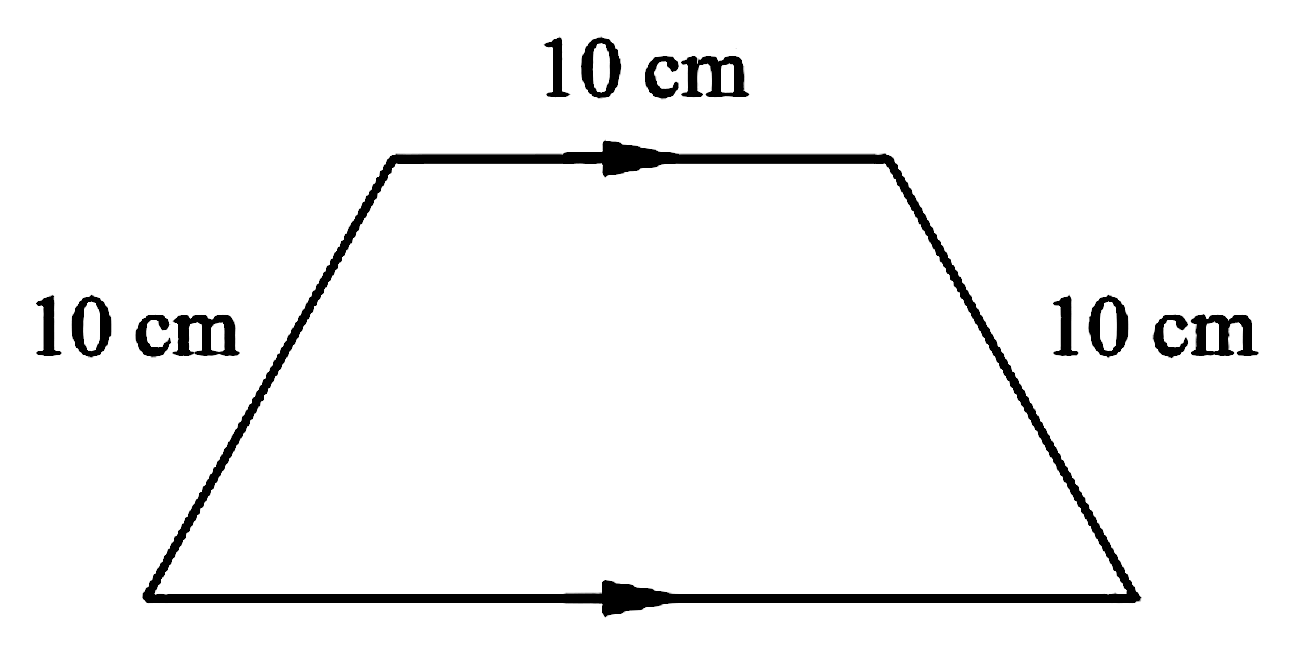
\includegraphics[scale=0.25]{assets/26-11.png}
          \end{center}
\end{enumerate}